% -*- root: ../paper.tex -*-

\begin{figure}
\centering
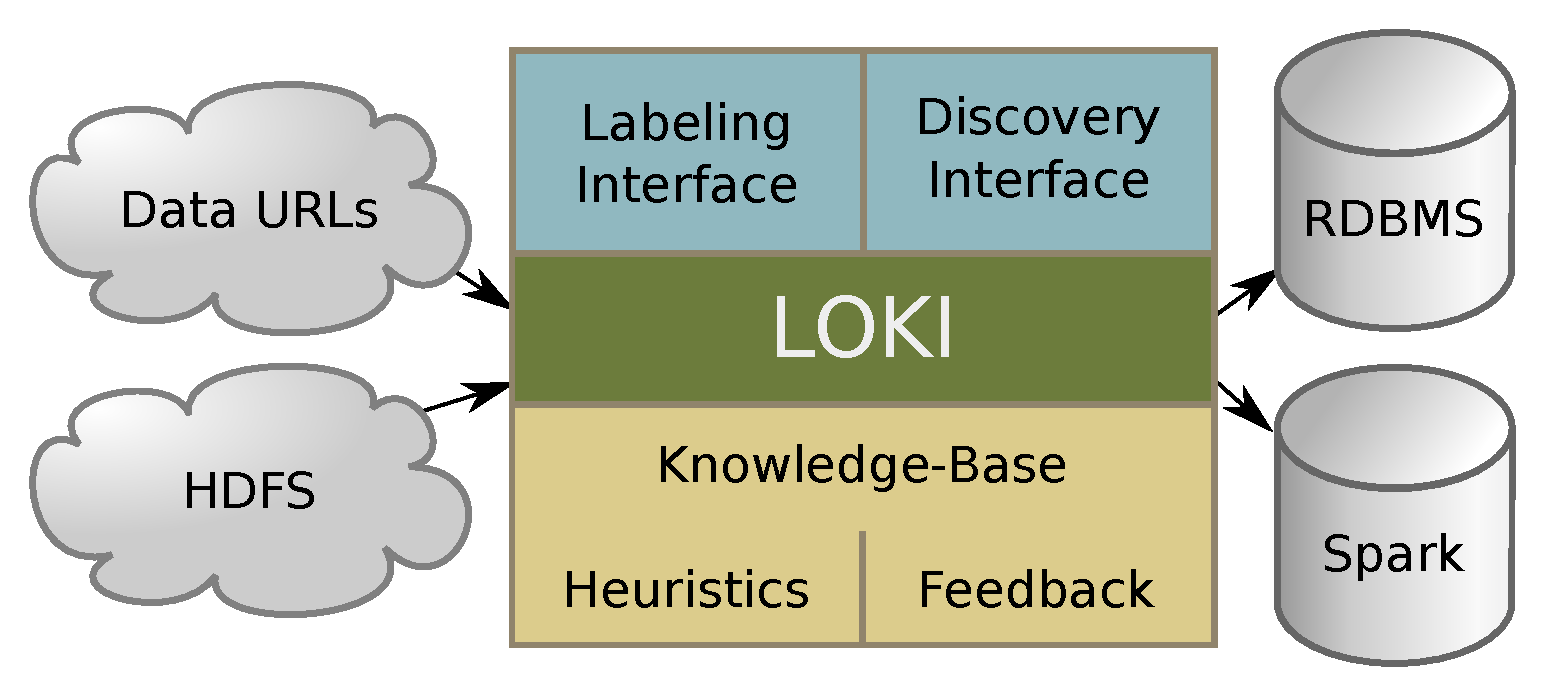
\includegraphics[width=0.8\columnwidth]{graphics/system.pdf}
\caption{System Overview}
\label{fig:overview}
\end{figure}

The overall goal of \systemname is to streamline the process of developing schemas for existing unlabeled or poorly labeled data sets.  
As illustrated in Figure~\ref{fig:overview}, \systemname lives alongside an existing RDBMS or Spark deployment, and takes as input tabular data in the form of a URL or HDFS file path.
\systemname provides users with two modes of interaction: (1) A \emph{labeling} interface that assists users in assigning names to existing columns of data, and (2) A \emph{discovery} interface that helps users to search for columns representing particular concepts of interest.  
Both interfaces are supported by a knowledge-base that combines expert-provided heuristics, learned characteristics, as well as historical feedback gathered from users about already-loaded datasets.
Once the user has labeled or discovered a sufficient set of columns, \systemname generates appropriate data loading/initialization code (e.g., a \texttt{CREATE TABLE} or Spark DataFrame initializer).  


\subsection{Labeling and Discovery}

We assume that data arrives in unlabeled tabular format.  
An input table $T$ has $N$ columns and consists of a set of rows $t \in T$.
Each row is an indexed list of attribute values $t = \tuple{t[1], \ldots, t[N]}$
With $1 \leq A \leq N$ we write $T_A$ to represent column $A$ of $T$, or the \emph{bag} of values located at that position in each row
$T_A = \bagcomprehension{t[A]}{t \in T}$.
We define the domain of $A$ in $T$, $dom_T(A)$ to be the \emph{set} of such values (i.e., $set(T_A)$).  
A \emph{schema} $S$ is a list of $N$ \emph{names}, or human interpretable strings $S[1], \ldots, S[N]$ identifying each attribute.
Note that this definition differs slightly from the classical definition of schemas, which here do not restrict the domain of a given attribute.

\systemname addresses two closely related problems that we term labeling and discovery.
For both, we assume the existence of a utility function $u(T_A, S[A]) \in [0, 1]$ that ranks the quality of a name $S[A]$ for a given column\footnote{Other factors might also be considered for the utility function (e.g., the rest of the schema or other columns of the table).  We leave these considerations for future work.}.  
Match-quality functions, discussed below, are one instance of this utility function.

\tinysection{Labeling}
In terms of the utility function, the goal of labeling is to take a table $T$ and infer a schema $S$ for it that maximizes total utility:
$$\argmax_{S}\left(\sum_{1 \leq A \leq N}u(T_A, S[A])\right)$$ 
optionally subject to the constraint that no two columns receive identical labels (i.e., for all $A \neq A'$, $S[A] \neq S[A']$).

\tinysection{Discovery}
We refer to the dual problem as discovery: Given a name $\namesymbol$, we would like to know which (if any) columns are valid candidates for $\namesymbol$:
$$\argmax_{A}\big(\; u(T_A, \namesymbol)\;\big)$$
optionally subject to a threshold value $0 \leq \delta \leq 1$ on the utility function.  We also consider the top-k variation of this problem, where we return the k columns with highest utility.

\subsection{Other Concerns}
In addition to the challenges of labeling and discovery, there are two additional challenges in implementing \systemname that, at present, we solve with off the shelf techniques.
First, \systemname need a way to infer the type (e.g., Numeric, String, or Ordinal) of columns of ingested data.  
For this, we adopt a simple counting-based technique~\cite{yang2015lenses}.
We attempt to parse each value using an array of regular expressions, one for each registered type.
A majority vote of successful parses in a column decides the column's type, with a threshold of 50\% indicating a string column and fewer than 100 distinct values indicating an ordinal.
Admittedly, more advanced techniques that relate columns, for example using functional dependencies, are possible.
However majority vote suffices for most use cases, and as such we leave more interesting type annotation schemes to future work.

Second, \systemname needs to load data into the underlying system.  
We use each platform's native loading scheme: \texttt{DataFrameReader}s on Spark, and native \texttt{LOAD} commands on RDBMSes, with a fall-back to manual \texttt{INSERT} operations if necessary.
As before, more intricate loading options are possible~\cite{DBLP:conf/sigmod/AlagiannisBBIA12,DBLP:conf/cidr/IdreosKM07}, but are beyond the scope of this paper.

\tinysection{User Interface}

\todo{Add some mockups of user interfaces for each of these}




